\documentclass[aspectratio=43]{beamer}

% Portada
\title{Diseño e implementación de módulos
funcionales (Sensores y Telemetría) de OBSW
para el desarrollo de nanosatélites}
\author{Jaime García González}
\institute{Universidad Carlos III de Madrid}
\date{4 de julio de 2019}
\titlegraphic{
\centering

\includegraphics[width=0.5\textwidth]{uc3m}

\includegraphics[width=0.25\textwidth]{sener}
}

% Tema
\usetheme[usetotalslideindicator]{metropolis}

% Fix tema
\makeatletter
\let\@@TOC=\tableofcontents
\def\tableofcontents[#1]{\bgroup\parskip=0pt\@@TOC[#1]\egroup}
\makeatother
\AtBeginDocument{
  \setbeamertemplate{section in toc}[square]
  \setbeamertemplate{itemize items}{\raisebox{.5ex}{\rule{.5ex}{.5ex}}}
  \fontsize{10}{15}\selectfont
}
\setbeamercovered{transparent}

% Barra de navegacion inferior
\setbeamertemplate{navigation symbols}{\vspace{-31pt}{%
  \insertslidenavigationsymbol\insertframenavigationsymbol%
  \insertsubsectionnavigationsymbol\insertsectionnavigationsymbol%
  \insertdocnavigationsymbol\insertbackfindforwardnavigationsymbol}}

% Transparencia inicio sección
\AtBeginSection{
\begin{frame}{Contenido}
  \tableofcontents[hidesubsections,currentsection]
\end{frame}
}

% Paquetes
\usepackage[spanish]{babel}
\usepackage[utf8]{luainputenc}
\usepackage{eurosym}
\usepackage{tikz}
\usetikzlibrary{chains}
\usepackage{pgfgantt}
\graphicspath{ {Figuras/} }

% Macros
\renewcommand\spanishtablename{Tabla}

\begin{document}

\maketitle

\begin{frame}{Contenido}
  \tableofcontents[hidesubsections]
\end{frame}

%% Capítulos
\section{Introducción}

% Descripción del proyecto

\begin{frame}{Descripción del proyecto (1/3)}

\begin{itemize}
\item Cátedra Universidad Carlos III - SENER.
\item Desarrollo de un nanosatélite universitario (Proyecto MARTÍN-LARA).
\item Tomar fotografías de la Tierra y estudiar los efectos de la radiación en componentes electrónicos.
\item Filosofía \emph{NewSpace}: Colonizar el espacio con nanosatélites y ofrecer nuevos servicios.
\end{itemize}

\end{frame}


\begin{frame}{Descripción del proyecto (2/3)}

\begin{figure}[h]
\centering
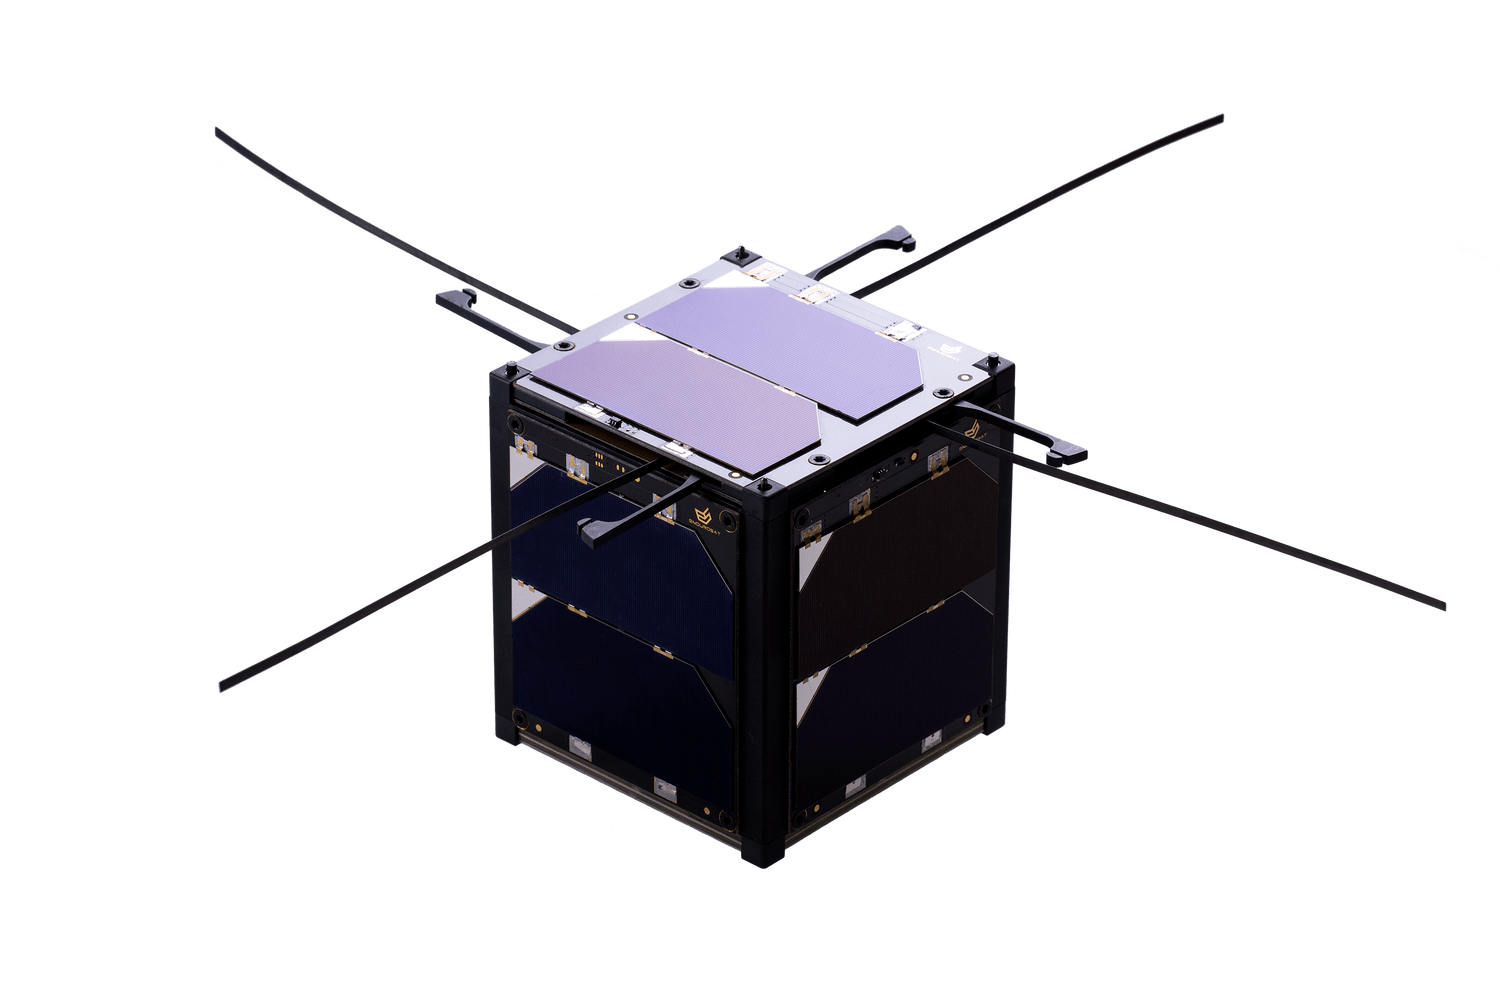
\includegraphics[width=0.4\textwidth]{cubesat}
\caption{\emph{CubeSat}. [Fuente: \texttt{https://satsearch.co/}]}
\end{figure}

Estándar \emph{CubeSat}:

\begin{itemize}
\item Desarrollar nanosatélites en aulas universitarias.
\item Restricciones de dimensiones ($10\times10\times10$ $cm$) y masa ($1.33$ $kg$).
\item Múltiples aplicaciones: observación de la Tierra, comunicaciones, IoT.
\end{itemize}

\end{frame}


\begin{frame}{Descripción del proyecto (3/3)}

\begin{columns}

\column{0.5\textwidth}
\vfill
La mayoría de estas misiones se componen de:

\begin{itemize}
\item Onboard Software (OBSW).
\item Ground System (GS).
\end{itemize}

\vspace{.1in}
Comunicación permanente mediante \emph{data link}.

\vfill

\column{0.5\textwidth}
\begin{figure}
\centering
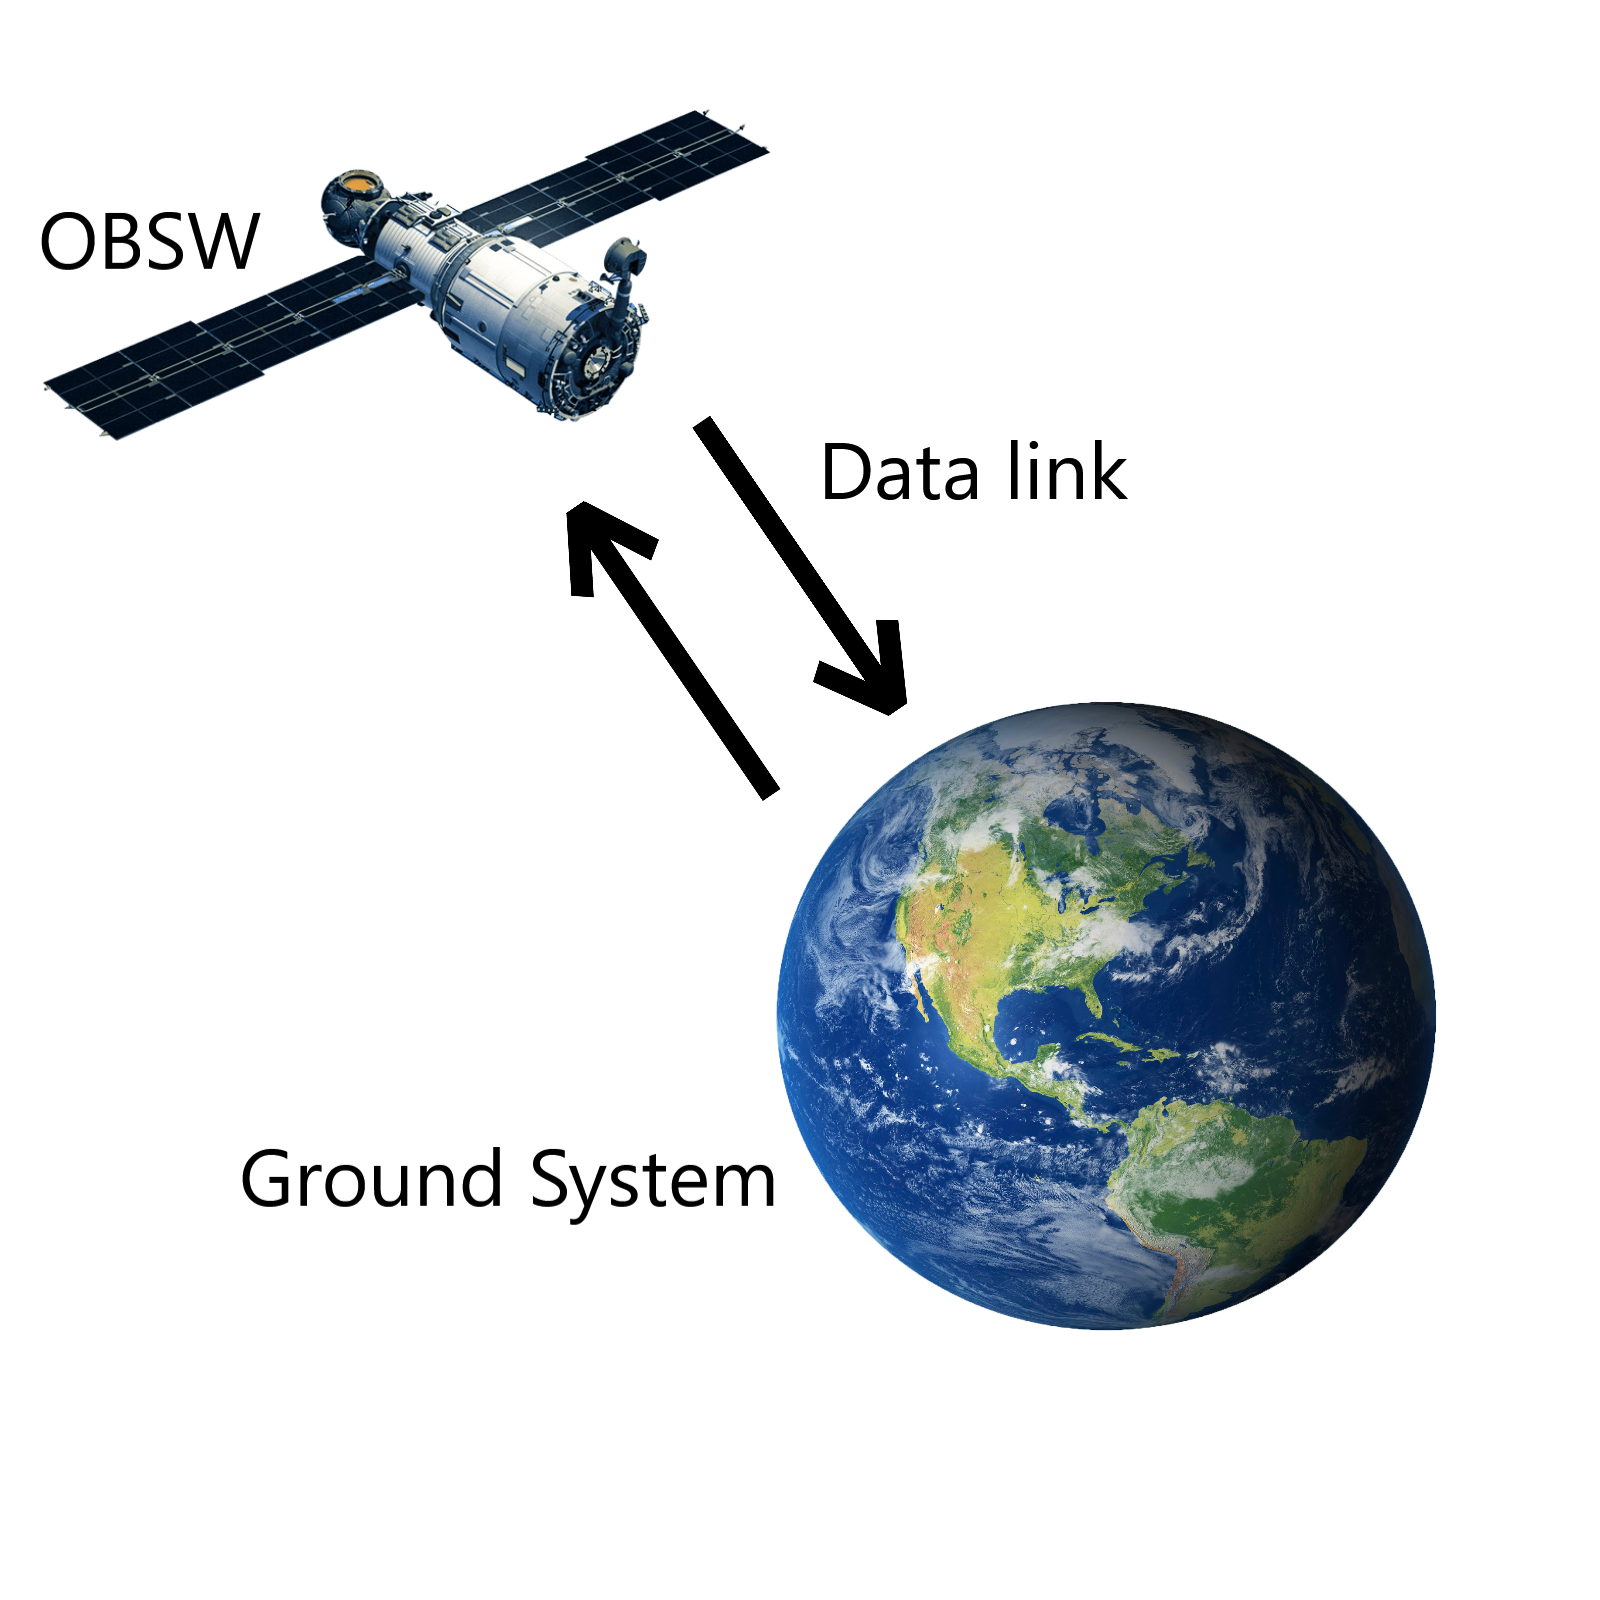
\includegraphics[width=0.9\textwidth]{dataLink}
\caption{\emph{Data link} entre OBSW y GS}
\end{figure}

\end{columns}

\end{frame}


% Motivación

\begin{frame}{Motivación}

El OBSW de estos nanosatélites se caracteriza por:

\begin{itemize}
\item \textbf{Modificación del entorno.} Reciben información del entorno utilizando sensores y modifican su estado con actuadores.
\item \textbf{Sistema crítico.} Ejecutado en un sistema operativo en tiempo real, RTOS. Dos premisas:

	\begin{enumerate}
		\item Ejecutar acciones correctas.
		\item Garantizar plazos de respuesta.
	\end{enumerate}

\end{itemize}

El incumplimiento de una de estas condiciones implica el \alert{fallo total} de la misión.

\end{frame}

% Objetivos

\begin{frame}{Objetivos}

\begin{enumerate}[<+->]
\item \textbf{Definición de la arquitectura del sistema.} Se participará en el diseño de la arquitectura global de la misión.
\item \textbf{Diseño e implementación del simulador térmico.} Definición, diseño e implementación de los diferentes componentes térmicos del sistema.
\item \textbf{Diseño e implementación del módulo de telemetría.} Definición e implementación de los paquetes transmitidos entre diferentes componentes del sistema.
\end{enumerate}

\end{frame}
\section{Análisis y diseño}

% cFE

\begin{frame}{Core Flight Executive (cFE)}

\begin{figure}
\center
\resizebox{!}{.33\textheight}{\begin{tikzpicture}[
	every node/.style={rectangle,font=\large,align=center,
	                   minimum height=0.66cm,text width=10cm,
	                   on chain,draw=olive!60!black!50},
	start chain=going above, node distance=8pt,
]

\node  [fill=olive!50!black!16] {Hardware};
\node  [fill=olive!50!black!14]  {Operating System (Linux, RTEMS, VxWorks, FreeRTOS)};
\node  [fill=olive!50!black!12] {Operating System Abstraction Layer (OSAL)};
\node  [fill=olive!50!black!10]  {cFE Services (Exec, Event, Bus, Table, Time)};
\node  [fill=olive!50!black!8] {cFS/User		Applications/Libraries};

\end{tikzpicture}}
\caption{Arquitectura sistema CFS}

\end{figure}

cFE es un OBSW desarrollado por NASA, que se caracteriza por:

\begin{itemize}
\item \emph{Framework} de desarrollo y entorno de ejecución.
\item Conjunto de servicios (Software Bus, Time, Events, etc).
\item Análisis de rendimiento en tiempo real.
\item Arquitectura modular.
\end{itemize}

\end{frame}


% Arquitectura global

\begin{frame}{Arquitectura de la misión}

\begin{figure}
\centering
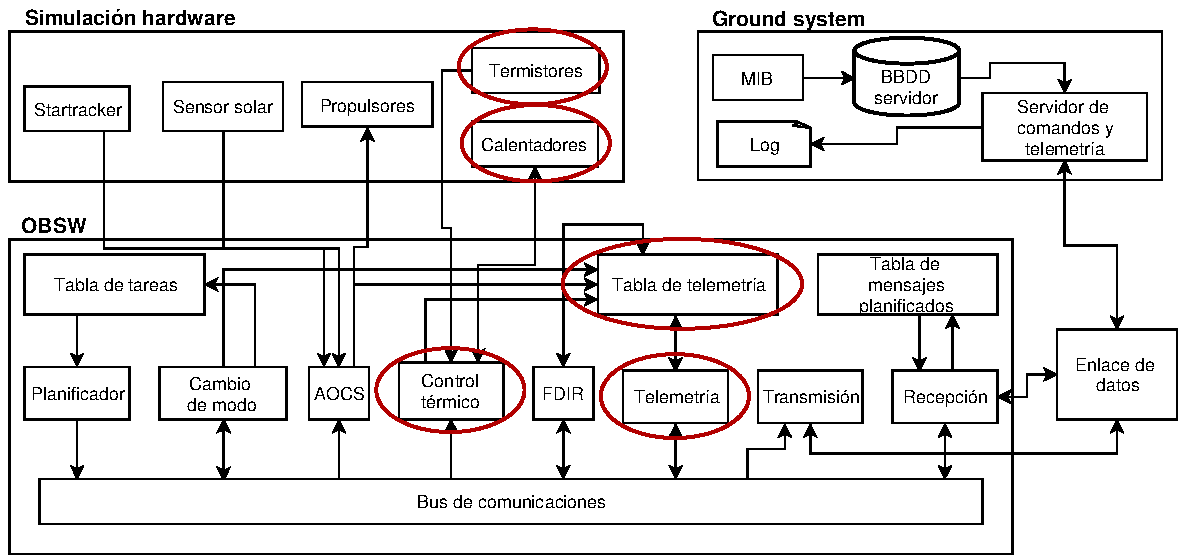
\includegraphics[width=\textwidth]{/arquitecturadelsistema}
\caption{Arquitectura de la misión}
\end{figure}

El sistema se compone de tres subsistemas:  Simulación hardware, OBSW y ground system.

\end{frame}


% Diagrama de componentes

\begin{frame}{Diseño de la solución}

\begin{figure}[h]
\centering
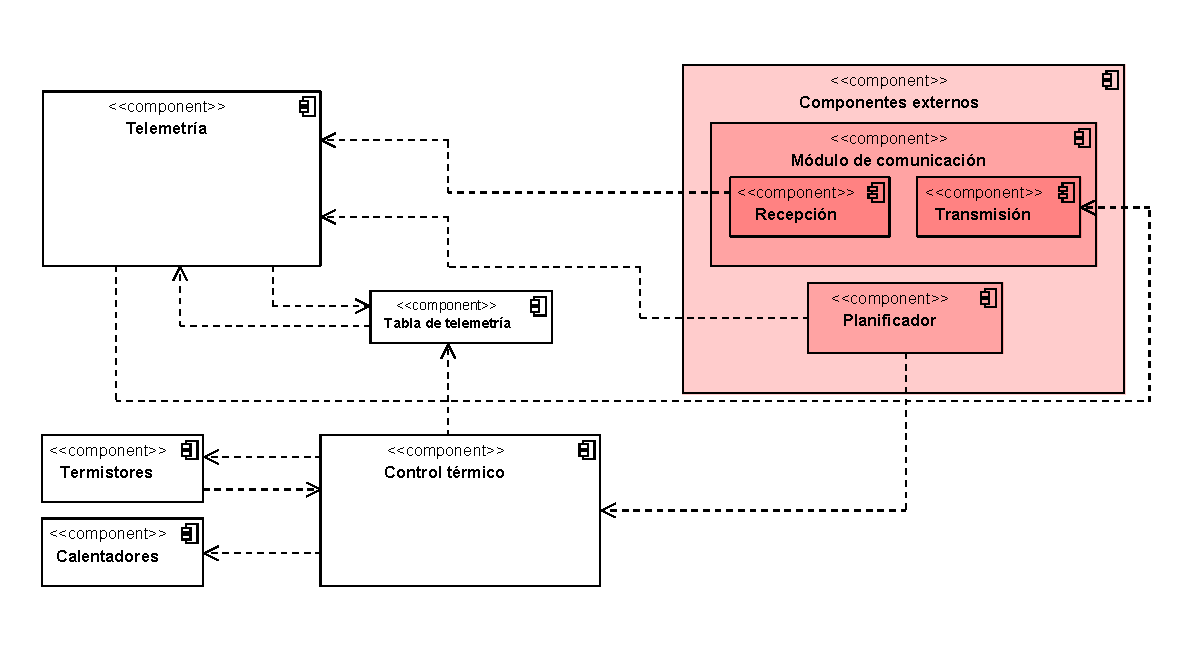
\includegraphics[width=\textwidth]{diagramacomponentes}
\caption{Diagrama de componentes}
\end{figure}

\end{frame}

\section{Implementación y pruebas}

% Introducción

\begin{frame}{Implementación}

Los componentes desarrollados se dividen en dos bloques:

\begin{itemize}[<+->]
\item \textbf{Módulo de telemetría.} Monitorizar el estado del sistema y enviar los paquetes al módulo de transmisión.
\item \textbf{Simulador térmico.} Control de la temperatura interna del sistema. Simulación software de componentes hardware.
\end{itemize}

\end{frame}

% Telemetría

\begin{frame}{Módulo de telemetría (1/2)}

\begin{figure}[h]
\centering
\resizebox{0.7\textwidth}{!}
{
\begin{tikzpicture} 
 		\draw [black] (0,0) rectangle (10,1);
        \draw [black] (0,0) rectangle (2,1)node[pos=.5] (Header) {Cabecera};  
        \draw [black] (2,0) rectangle (10,1) node[pos=.5] (user) {Segmento de datos};       
        
\end{tikzpicture}
}
\caption{Estructura de paquete}
\end{figure}

\begin{itemize}
\item \textbf{Cabecera.} Identificador de paquete, \emph{checksum} y \emph{timestamp}.
\item \textbf{Segmento de datos.} Valores de sensores, actuadores y control del sistema.
\end{itemize}


Principales características:

\begin{itemize}
\item Evitar números en coma flotante (errores de precisión).
\item Reducir \emph{overhead} en sistemas empotrados.
\item Optimización de espacio empaquetando indicadores binarios en una variable de 32 bits.
\end{itemize}

\end{frame}


\begin{frame}{Módulo de telemetría (2/2)}

\begin{figure}
\centering
\resizebox{0.82\textwidth}{!}
{
\begin{tikzpicture} 
 		\draw [black] (0,0) rectangle (14,1);
 		\draw [black] (0,0) rectangle (1,1)node[pos=.5] () {31};  
        \draw [black] (1,0) rectangle (2,1)node[pos=.5] () {30};  
         \draw [black] (2,0) rectangle (3,1)node[pos=.5] () {29};  
         \draw [black] (3,0) rectangle (4,1)node[pos=.5] () {28};  
          \draw [black] (4,0) rectangle (12,1)node[pos=.5] () {\ldots};  
           \draw [black] (12,0) rectangle (13,1)node[pos=.5] () {1};  
           \draw [black] (13,0) rectangle (14,1)node[pos=.5] () {0};  
             
        
       
\end{tikzpicture}
}
\caption{Empaquetado de indicadores binarios}
\end{figure}

\begin{columns}

\column{0.5\textwidth}

\begin{center}
\textbf{Paquete periódico}
\end{center}

\begin{itemize}
\item Envío periódico (0.2 Hz).
\item Toda la información del sistema.
\item Incluye \emph{flags} de estado.
\end{itemize}

\column{0.5\textwidth}

\begin{center}
\textbf{Paquete puntual}
\end{center}

\begin{itemize}
\item Envío $\Leftrightarrow$ solicitud del GS.
\item Diferentes tipos de paquetes (térmico, posicional y solar).
\item Incluye \emph{flags} de estado.
\end{itemize}

\end{columns}

\end{frame}


% Simulador térmico

\begin{frame}{Simulador térmico (1/2)}

Simulación software de los componentes térmicos del nanosatélite y módulo del OBSW.

\begin{itemize}[<+->]
\item \textbf{Calentadores.} Simulan un aumento de la temperatura.
\item \textbf{Termistores.} Simulan una lectura de temperatura.

\begin{center}
$T(t) = \mathcal{C} + A*sin(2\Pi\upsilon t + \varphi)$
\end{center}

\begin{figure}
\resizebox{0.8\textwidth}{!}{
 \begin{tikzpicture}
    \draw (0,0) -- (12,0);
    \draw (0.2,1)node[left,font=\tiny] {$y=233 K$} -- (11.8,1);
    \draw (0.2,-1)node[left,font=\tiny] {$y=203 K$} -- (11.8,-1); 
    \draw (0,0)node [left,font=\tiny,] {$\mathcal{C} = 218 K$};
    
    \draw (0,-0.2)node [below,font=\tiny,] {0} -- (0,0.2) ;
    \draw (4,-0.2)node [below,font=\tiny,] {300} -- (4,0.2) ;
    \draw (8,-0.2)node [below,font=\tiny,] {600} -- (8,0.2) ;
    \draw (12,-0.2)node [below,font=\tiny,] {900} -- (12,0.2) ;

    \draw[ultra thick, red] (0,0) sin (1,1);
    \draw[ultra thick, red] (1,1) cos (2,0);
    \draw[ultra thick, red] (2,0) sin (3,-1);
    \draw[ultra thick, red] (3,-1) cos (4,0);
    \draw[ultra thick, red] (4,0)  sin (5,1);
    \draw[ultra thick, red] (5,1) cos (6,0);
    \draw[ultra thick, red] (6,0) sin (7,-1);
    \draw[ultra thick, red] (7,-1) cos (8,0);
    \draw[ultra thick, red] (8,0) sin (9,1);
    \draw[ultra thick, red] (9,1) cos (10,0);
    \draw[ultra thick, red] (10,0) sin (11,-1);
    \draw[ultra thick, red] (11,-1) cos (12,0);
    \end{tikzpicture}
}  

\caption{Simulación lectura de temperatura}  
\end{figure}

\end{itemize}

\end{frame}


\begin{frame}{Simulador térmico (2/2)}

\begin{itemize}
\item \textbf{Control térmico.} Módulo de OBSW que controla la temperatura interna del sistema. 
\end{itemize}

Verifica los umbrales de temperatura de cada termistor y enciende/apaga su calentador asociado.

\begin{center}
$Termistor \rightarrow verificar$ $umbrales \rightarrow calentador$
\end{center}

Para lograr una simulación real, se añade un factor de ruido.

\begin{center}
$T_{i} = Thermistor_{i} + rand (-2,2) \mid \forall i \subset \{1,2,3\}$
\end{center}
 
\end{frame}


% Pruebas y evaluación

\begin{frame}{Pruebas y evaluación (1/2)}

Pruebas de verificación e integración para todos los componentes desarrollados.

\begin{columns}

\column{0.5\textwidth}

\begin{center}
\textbf{Entorno de pruebas}
\end{center}

\begin{itemize}
\item Intel Core i7 - 2.60 GHz.
\item 12 GB RAM DDR3.
\end{itemize}

\column{0.5\textwidth}

\begin{center}
\textbf{Sistema final}
\end{center}

\begin{itemize}
\item ARM Cortex A8 - 1 GHz.
\item 512 MB LPDDR RAM.
\end{itemize}

\end{columns}

\vspace{0.1 in}

Intervalo de confianza para comprobar que se cumplen las restricciones temporales.

\begin{figure}
$\mu = \bar{x}  \pm z {\sigma \over \sqrt{n}}$
\end{figure}

\end{frame}


\begin{frame}{Pruebas y evaluación (2/2)}

\begin{table}[h]
\centering
\resizebox{0.85\textwidth}{!}{
		\begin{tabular}{|c|c|c|c|}
		\hline 
		Módulo & Cómputo máximo (ms) & Cota inferior (ms) & Cota superior (ms)\\
		\hline
		Telemetría & 31.25 & 0.0168  & 0.0186 \\
		\hline
		Control térmico &  31.25 & 0.0162  & 0.0705\\	
		\hline
		\end{tabular}
		}
		\caption{Intervalo de confianza}
\end{table}

\begin{columns}

\column{0.5\textwidth}

\begin{figure}[h]
\centering
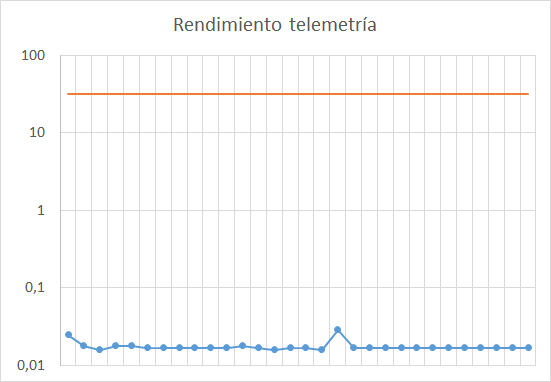
\includegraphics[width=0.98\textwidth]{rendimiento1}
\caption{Rendimiento telemetría}
\end{figure}

\column{0.5\textwidth}

\begin{figure}[h]
\centering
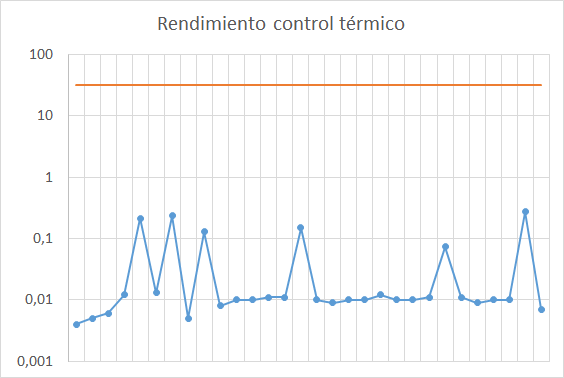
\includegraphics[width=\textwidth]{rendimiento2}
\caption{Rendimiento c. térmico}
\end{figure}

\end{columns}

\end{frame}
\section{Plan de proyecto}

% Gantt de proyecto
\begin{frame}{Planificación}
\resizebox{!}{.72\textheight}{
 \begin{ganttchart}[y unit title=0.7cm,y unit chart=0.6cm,x unit= 0.7 mm, 			hgrid=true, time slot format={little-endian}]{14.09.2018}{30.06.2019} 
  
	\gantttitlecalendar{year, month=shortname} \\
	
	\ganttmilestone{Presentación del proyecto}{14.09.2018}\\

	\ganttmilestone{Inicio del proyecto}{16.10.2018}\\ 
  
	% Planificacion proyecto
	\ganttgroup{Planificación}{16.10.2018}{20.11.2018} \\
	\ganttbar{Lectura documentación}{16.10.2018}{27.10.2018}\\
	\ganttbar{Estudio cFE}{23.10.2018}{02.11.2018} \\
	\ganttbar{Herramientas alternativas}{04.11.2018}{13.11.2018}\\
 
	% Analisis del sistema y requisitos  
	\ganttgroup{Análisis y diseño}{20.11.2018}{21.12.2018} \\
	\ganttbar{Definición de requisitos}{20.11.2018}{05.12.2018} \\
	\ganttbar{Diseño del sistema}{08.12.2018}{21.12.2018} \\
	
	% Implementacion	
	\ganttgroup{Implementación}{21.12.2018}{06.04.2019} \\
	\ganttbar{Simulador térmico}{21.12.2018}{20.01.2019}\\
	\ganttbar{Módulo de telemetría}{24.01.2019}{27.02.2019} \\
	\ganttbar{Integración}{08.03.2019}{06.04.2019} \\

	% Pruebas
	\ganttgroup{Pruebas y evaluación}{06.04.2019}{18.04.2019} \\
	\ganttbar{Pruebas}{06.04.2019}{13.04.2019}\\
	\ganttbar{Evaluación del sistema}{14.04.2019}{18.04.2019}\\
	
	% Documentacion
	\ganttgroup{Documentación}{24.04.2019}{10.06.2019}\\
	\ganttbar{Memoria}{24.04.2019}{04.06.2019}\\
	\ganttbar{Presentación}{06.06.2019}{10.06.2019}\\
	
	
	\ganttmilestone{Entrega del proyecto}{17.06.2019}\\ 
	
	%Grupos
	\ganttlink{elem1}{elem2}
	\ganttlink{elem2}{elem6}
	\ganttlink{elem6}{elem9}
	\ganttlink{elem9}{elem13}
	\ganttlink{elem13}{elem16}
	
	
	%%Tareas
	\ganttlink{elem7}{elem8}
	\ganttlink{elem10}{elem11}
	\ganttlink{elem11}{elem12}	
	\ganttlink{elem17}{elem18}
	\ganttlink{elem17}{elem19}

	
  \end{ganttchart}
  }

\end{frame}


% Presupuesto

\begin{frame}{Presupuesto}

El proyecto ha tenido una duración aproximada de \textbf{8 meses}. El coste total del mismo asciende a \textbf{14931.47 \euro }.

\begin{table}[h]
\centering
		\begin{tabular}{|l|r|}
		\hline 
		Descripción & Coste\\
		\hline
		\hline
		Costes de personal & 8560.00 \euro  \\
		\hline		
		Amortización & 132.13 \euro  \\
		\hline
		Costes indirectos & 282.10  \euro \\
		\hline
		Margen de imprevistos (10 \%{}) & 897.46 \euro  \\
		\hline 
		Margen de beneficio (25 \%{}) & 2468.02 \euro  \\
		\hline
		\hline
		Total sin I.V.A. & 12340.06 \euro \\
		\hline
		\hline
		\textbf{Total} & \textbf{14931.47 \euro } \\		
		\hline
		\end{tabular}
		\caption{Resumen de costes}
\end{table}

\end{frame}

% Marco legal

\begin{frame}{Marco legal}

El proyecto está sujeto a las siguientes leyes/normativas:

\begin{itemize}
\item \textbf{Tratado sobre el espacio exterior.} Control de actividades espaciales de los Estados, registro de lanzamientos, etc. 
\item \textbf{CCSDS.} Desarrollo de estándares para misiones espaciales.
\item \textbf{ECSS.} Desarrollo de estándares para misiones espaciales a nivel europeo.
\item \textbf{CNAF.} Control de radiofrecuencias en el territorio nacional.
\end{itemize}

\end{frame}
\section{Conclusiones y trabajo futuro}

% Conclusiones

\begin{frame}{Conclusiones}

\begin{itemize}[<+->]
\item \textbf{Arquitectura del sistema.} Arquitectura modular, componentes independientes, fácil mantenimiento y desarrollo.
\item \textbf{Simulador térmico.} Simulación de lectura y aumento de temperatura. Control de la temperatura interna del sistema.
\item \textbf{Módulo de telemetría.} Definición e implementación de paquetes periódicos y puntuales. Optimización de espacio, evitando pérdida de precisión. Adaptado para sistemas empotrados.

\end{itemize}

\end{frame}


% Trabajo futuro

\begin{frame}{Trabajo futuro}

Primer año de la Cátedra UC3M - SENER, trabajo a realizar en siguientes iteraciones:

\begin{itemize}
\item \textbf{Integración con Simulink.} Simulación con modelos reales (\emph{model-in-the-loop}).
\item \textbf{Gestión de memoria.} Nuevos paquetes, corrección de errores, nueva funcionalidad (\emph{payloads}).
\item \textbf{Documentación.} Generar documentación del código con Doxygen.
\item \textbf{Sensores/actuadores.} Nuevos componentes que complementen la misión.
\end{itemize}

\end{frame}
\maketitle

\end{document}
